% This template has been tested with IEEEtran of 2015.

% !TeX spellcheck = en-US
% LTeX: language=en-US
% !TeX encoding = utf8
% !TeX program = luatex
% !BIB program = bibtex
% -*- coding:utf-8 mod:LaTeX -*-


\documentclass[journal,letterpaper,english]{IEEEtran}[2015/08/26]

% Balance the last page using the balance package (see https://ctan.org/pkg/balance)
% Alternative to balance is the pbalance package (see https://ctan.org/pkg/pbalance), which sometimes works better
\usepackage{balance}
%\usepackage{pbalance}

\usepackage{iftex}
% backticks (`) are rendered as such in verbatim environments.
% See following links for details:
%   - https://tex.stackexchange.com/a/341057/9075
%   - https://tex.stackexchange.com/a/47451/9075
%   - https://tex.stackexchange.com/a/166791/9075
\usepackage{upquote}

% Set English as language and allow to write hyphenated"=words
%
% Even though `american`, `english` and `USenglish` are synonyms for babel package (according to https://tex.stackexchange.com/questions/12775/babel-english-american-usenglish), the llncs document class is prepared to avoid the overriding of certain names (such as "act." -> "Abstract" or "Fig." -> "") when using `english`, but not when using the other 2.
% english has to go last to set it as default language
\usepackage[ngerman,main=english]{babel}
%
% Hint by http://tex.stackexchange.com/a/321066/9075 -> enable "= as dashes
\addto\extrasenglish{\languageshorthands{ngerman}\useshorthands{"}}

% Links behave as they should. Enables "\url{...}" for URL typesettings.
% Allow URL breaks also at a hyphen, even though it might be confusing: Is the "-" part of the address or just a hyphen?
% See https://tex.stackexchange.com/a/3034/9075.
\usepackage[hyphens]{url}

% When activated, use text font as url font, not the monospaced one.
% For all options see https://tex.stackexchange.com/a/261435/9075.
\urlstyle{same}

% Improve wrapping of URLs - hint by http://tex.stackexchange.com/a/10419/9075
\makeatletter
\g@addto@macro{\UrlBreaks}{\UrlOrds}
\makeatother

% nicer // - solution by http://tex.stackexchange.com/a/98470/9075
% DO NOT ACTIVATE -> prevents line breaks
%\makeatletter
%\def\Url@twoslashes{\mathchar`\/\@ifnextchar/{\kern-.2em}{}}
%\g@addto@macro\UrlSpecials{\do\/{\Url@twoslashes}}
%\makeatother

% Modern replacement for Times.sty that sets math fonts correctly and scales helvet properly
\usepackage{mathptmx}
\usepackage[scaled=.90]{helvet}
\usepackage{courier}

%% !! Include math libraries before unicode-math
\usepackage{amsmath}
\interdisplaylinepenalty=2500 
\usepackage{amssymb}
\usepackage{mathtools}
\usepackage{lualatex-math}
\usepackage{xfrac}
\usepackage{mdwmath}
\usepackage{cases}


%% !!! If you change the font, be sure that words such as "workflow" can
%% !!! still be copied from the PDF. If this is not the case, you have
%% !!! to use glyphtounicode. See comment at cmap package.
%%
%% Background: "workflow" contains "fl" which is a ligature, which in turn
%%             is rendered as one character in the PDF and needs to be split
%%             whily copying.

\ifluatex
  \usepackage[no-math]{fontspec}
  \defaultfontfeatures{Ligatures = TeX}

  \usepackage{unicode-math}

  % Enable proper ligatures
  % For more information see https://ctan.org/pkg/selnolig
  % language "english" or "ngerman" is passed to selnolig by the document class
  \usepackage{selnolig}
  
  \setmonofont[Scale=0.82]{Cascadia Mono}
%  \setmonofont{Courier New}
%  \setmainfont{Times New Roman}
%  \setmainfont{TeX Gyre Termes}
%    \setmainfont{Times}
    \setmathfont{STIX Two Math}[
    Extension={.otf},
    Path=./stixfonts/fonts/static_otf/,
    Scale=1]
    \setmainfont{Stix Two Text}[
    Extension={.otf},
    Path=./stixfonts/fonts/static_otf/,
    UprightFont={*-Regular},
    BoldFont={*-Bold},
    ItalicFont={*-Italic},
    BoldItalicFont={*-BoldItalic}]
\else
\defaultfontfeatures{Ligatures = TeX, Mapping = tex-text}
  % use nicer font for code
  \usepackage[zerostyle=b,scaled=.75]{newtxtt}

  % Has to be loaded AFTER any font packages. See https://tex.stackexchange.com/a/2869/9075.
  \usepackage[T1]{fontenc}
\fi

\usepackage{ninecolors}

% Character protrusion and font expansion. See http://www.ctan.org/tex-archive/macros/latex/contrib/microtype/


\usepackage[section]{placeins}

% \texttt{test -- test} keeps the "--" as "--" (and does not convert it to an en dash)
\ifLuaTeX
\usepackage[
babel=true, % Enable language-specific kerning. Take language-settings from the languge of the current document (see Section 6 of microtype.pdf)
expansion=alltext,
protrusion=alltext-nott, % Ensure that at listings, there is no change at the margin of the listing
% In the standard configuration, this template is always in the final mode, so this option only makes a difference if "pros" use the draft mode
final % Always enable microtype, even if in draft mode. This helps finding bad boxes quickly.
]{microtype}
\DisableLigatures{encoding = T1, family = tt* }
\else\ifPDFTeX
\usepackage[
babel=true, % Enable language-specific kerning. Take language-settings from the languge of the current document (see Section 6 of microtype.pdf)
expansion=alltext,
protrusion=alltext-nott, % Ensure that at listings, there is no change at the margin of the listing
% In the standard configuration, this template is always in the final mode, so this option only makes a difference if "pros" use the draft mode
final % Always enable microtype, even if in draft mode. This helps finding bad boxes quickly.
]{microtype}
\DisableLigatures{encoding = T1, family = tt* }
\fi
\fi


%\DeclareMicrotypeSet*[tracking]{my}{ font = */*/*/sc/* }%
%\SetTracking{ encoding = *, shape = sc }{ 45 }
% Source: http://homepage.ruhr-uni-bochum.de/Georg.Verweyen/pakete.html
% Deactiviated, because does not look good

\usepackage{graphicx}

% Diagonal lines in a table - http://tex.stackexchange.com/questions/17745/diagonal-lines-in-table-cell
% Slashbox is not available in texlive (due to licensing) and also gives bad results. Thus, we use diagbox
\usepackage{diagbox}

\ifluatex
  \usepackage{spelling}
  \spellingoutput{off}
\fi

\usepackage[dvipsnames, table]{xcolor}
% Code Listings
\usepackage{listings}

\definecolor{eclipseStrings}{RGB}{42,0,255}
\definecolor{eclipseKeywords}{RGB}{127,0,85}
\definecolor{spiceComment}{RGB}{0,128,0}
\definecolor{spiceDotCommand}{RGB}{0,0,255}
\definecolor{spiceContinuationText}{RGB}{255,0,0}
\colorlet{numb}{magenta!60!black}
\colorlet{back-color}{gray9!30!white}

\definecolor{main-color}{rgb}{0.6627, 0.7176, 0.7764}


% SPICE definition
% CUSTOM
\lstdefinelanguage{spice}{
	escapeinside={;(*}{*)},
	basicstyle=\normalfont\scriptsize\ttfamily,
	commentstyle=\color{spiceComment}, % style of comment
	numbers=left,
	stringstyle=\textrm\color{eclipseKeywords}, % style
	string=[s]{"}{"},
	numberstyle=\tiny\ttfamily\color{black},
%	showspaces=true,
%	showtabs=true,
	stepnumber=1,
	breaklines=true,
	breakatwhitespace=true,
	columns=fixed,
	numbersep=8pt,
%	showstringspaces=true,
	breaklines=true,
%	frame=lines,
	backgroundcolor=\color{back-color},
	sensitive=false,
	comment=[l]{\;},
	morecomment=[l]{*},
	moredelim=[l][\color{spiceContinuationText}]{+},
	moredelim=[l][\color{spiceDotCommand}]{.},
}


% JSON definition
% Source: https://tex.stackexchange.com/a/433961/9075

\lstdefinelanguage{json}{
  basicstyle=\normalfont\footnotesize\ttfamily,
  commentstyle=\color{eclipseStrings}, % style of comment
  stringstyle=\color{eclipseKeywords}, % style of strings
  numbers=left,
  numberstyle=\scriptsize,
  stepnumber=1,
  numbersep=8pt,
  showstringspaces=false,
  breaklines=true,
  frame=lines,
%  backgroundcolor=\color{gray}, %only if you like
  string=[s]{"}{"},
  comment=[l]{:\ "},
  morecomment=[l]{:"},
  literate=
    *{0}{{{\color{numb}0}}}{1}
    {1}{{{\color{numb}1}}}{1}
    {2}{{{\color{numb}2}}}{1}
    {3}{{{\color{numb}3}}}{1}
    {4}{{{\color{numb}4}}}{1}
    {5}{{{\color{numb}5}}}{1}
    {6}{{{\color{numb}6}}}{1}
    {7}{{{\color{numb}7}}}{1}
    {8}{{{\color{numb}8}}}{1}
    {9}{{{\color{numb}9}}}{1}
}



\lstset{
  showstringspaces=false,
  extendedchars=true,
  basicstyle=\footnotesize\ttfamily,
  commentstyle=\slshape
  numberstyle=\tiny\ttfamily\color{black},
  stepnumber=1,
  breaklines=true,
  breakatwhitespace=true,
  columns=fixed,
  numbersep=8pt,
  breaklines=true,
  frame=lines,
  tabsize=2,                  % Groesse von Tabs
  numbers=left,
  basewidth=.5em,
  xleftmargin=.5cm,
  % aboveskip=0mm,
  % belowskip=0mm,
  captionpos=b
}


\lstloadlanguages{% Check dokumentation for further languages...
  %[Visual]Basic
  %Pascal
  %C
  %C++
  %XML
  %HTML
  Python,
  Octave
}



\definecolor{checkboxBorder}{RGB}{145,145,145}%"#919191"
\definecolor{editorBackground}{RGB}{255,255,255}%"#FFFFFF"
\definecolor{editorForeground}{RGB}{0,0,0}%"#000000"
\definecolor{editorInactiveselectionbackground}{RGB}{229,235,241}%"#E5EBF1"
\definecolor{editorindentguideBackground1}{RGB}{211,211,211}%"#D3D3D3"
\definecolor{editorindentguideActivebackground1}{RGB}{147,147,147}%"#939393"
\definecolor{editorSelectionhighlightbackground}{RGB}{173,214,255}%"#ADD6FF80"
\definecolor{editorsuggestwidgetBackground}{RGB}{243,243,243}%"#F3F3F3"
\definecolor{activitybarbadgeBackground}{RGB}{0,122,204}%"#007ACC"
\definecolor{sidebartitleForeground}{RGB}{111,111,111}%"#6F6F6F"
\definecolor{listHoverbackground}{RGB}{232,232,232}%"#E8E8E8"
\definecolor{menuBorder}{RGB}{212,212,212}%"#D4D4D4"
\definecolor{inputPlaceholderforeground}{RGB}{118,118,118}%"#767676"
\definecolor{searcheditorTextinputborder}{RGB}{206,206,206}%"#CECECE"
\definecolor{settingsTextinputborder}{RGB}{206,206,206}%"#CECECE"
\definecolor{settingsNumberinputborder}{RGB}{206,206,206}%"#CECECE"
\definecolor{statusbaritemRemoteforeground}{RGB}{255,255,255}%"#FFF"
\definecolor{statusbaritemRemotebackground}{RGB}{22,130,93}%"#16825D"
\definecolor{portsIconrunningprocessforeground}{RGB}{54,148,50}%"#369432"
\definecolor{sidebarsectionheaderBackground}{RGB}{0,0,0}%"#0000"
\definecolor{sidebarsectionheaderBorder}{RGB}{97,97,97}%"#61616130"
\definecolor{tabSelectedforeground}{RGB}{51,51,51}%"#333333b3"
\definecolor{tabSelectedbackground}{RGB}{255,255,255}%"#ffffffa5"
\definecolor{tabLastpinnedborder}{RGB}{97,97,97}%"#61616130"
\definecolor{notebookCellbordercolor}{RGB}{232,232,232}%"#E8E8E8"
\definecolor{notebookSelectedcellbackground}{RGB}{200,221,241}%"#c8ddf150"
\definecolor{statusbaritemErrorbackground}{RGB}{199,46,15}%"#c72e0f"
\definecolor{listActiveselectioniconforeground}{RGB}{255,255,255}%"#FFF"
\definecolor{listFocusandselectionoutline}{RGB}{144,194,249}%"#90C2F9"
\definecolor{terminalInactiveselectionbackground}{RGB}{229,235,241}%"#E5EBF1"
\definecolor{widgetBorder}{RGB}{212,212,212}%"#d4d4d4"
\definecolor{actionbarToggledbackground}{RGB}{221,221,221}%"#dddddd"
\definecolor{diffeditorUnchangedregionbackground}{RGB}{248,248,248}%"#f8f8f8"
\definecolor{newOperator}{RGB}{0,0,255}%"#0000ff"
\definecolor{stringLiteral}{RGB}{163,21,21}%"#a31515"
\definecolor{customLiteral}{RGB}{0,0,0}%"#000000"
\definecolor{numberLiteral}{RGB}{9,134,88}%"#098658"
\definecolor{variableLegacyBuiltinPython}{RGB}{0,0,0}%"#000000ff"
\definecolor{metaDiffHeader}{RGB}{0,0,128}%"#000080"
\definecolor{comment}{RGB}{0,128,0}%"#008000"
\definecolor{constantLanguage}{RGB}{0,0,255}%"#0000ff"
\definecolor{keywordOperatorMinusExponent}{RGB}{9,134,88}%"#098658"
\definecolor{constantRegexp}{RGB}{129,31,63}%"#811f3f"
\definecolor{cssTagsInSelectorsXmlTags}{RGB}{128,0,0}%"#800000"
\definecolor{entityNameSelector}{RGB}{128,0,0}%"#800000"
\definecolor{entityOtherAttributeName}{RGB}{229,0,0}%"#e50000"
\definecolor{entityOtherAttributeNameScss}{RGB}{128,0,0}%"#800000"
\definecolor{invalid}{RGB}{205,49,49}%"#cd3131"
\definecolor{markupBold}{RGB}{0,0,128}%"#000080"
\definecolor{markupHeading}{RGB}{128,0,0}%"#800000"
\definecolor{markupInserted}{RGB}{9,134,88}%"#098658"
\definecolor{markupDeleted}{RGB}{163,21,21}%"#a31515"
\definecolor{markupChanged}{RGB}{4,81,165}%"#0451a5"
\definecolor{punctuationDefinitionListBeginMarkdown}{RGB}{4,81,165}%"#0451a5"
\definecolor{markupInlineRaw}{RGB}{128,0,0}%"#800000"
\definecolor{bracketsOfXmlhtmlTags}{RGB}{128,0,0}%"#800000"
\definecolor{entityNameFunctionPreprocessor}{RGB}{0,0,255}%"#0000ff"
\definecolor{metaPreprocessorString}{RGB}{163,21,21}%"#a31515"
\definecolor{metaPreprocessorNumeric}{RGB}{9,134,88}%"#098658"
\definecolor{metaStructureDictionaryKeyPython}{RGB}{4,81,165}%"#0451a5"
\definecolor{storage}{RGB}{0,0,255}%"#0000ff"
\definecolor{storageType}{RGB}{0,0,255}%"#0000ff"
\definecolor{keywordOperatorNoexcept}{RGB}{0,0,255}%"#0000ff"
\definecolor{metaEmbeddedAssembly}{RGB}{163,21,21}%"#a31515"
\definecolor{stringQuotedDoubleHandlebars}{RGB}{0,0,255}%"#0000ff"
\definecolor{stringRegexp}{RGB}{129,31,63}%"#811f3f"
\definecolor{stringInterpolation}{RGB}{0,0,255}%"#0000ff"
\definecolor{resetJavascriptStringInterpolationExpression}{RGB}{0,0,0}%"#000000"
\definecolor{supportConstantColor}{RGB}{4,81,165}%"#0451a5"
\definecolor{sourceCoffeeEmbedded}{RGB}{229,0,0}%"#e50000"
\definecolor{supportTypePropertyNameJson}{RGB}{4,81,165}%"#0451a5"
\definecolor{keyword}{RGB}{0,0,255}%"#0000ff"
\definecolor{keywordControl}{RGB}{0,0,255}%"#0000ff"
\definecolor{keywordOperator}{RGB}{0,0,0}%"#000000"
\definecolor{keywordOperatorWordlike}{RGB}{0,0,255}%"#0000ff"
\definecolor{keywordOtherUnit}{RGB}{9,134,88}%"#098658"
\definecolor{punctuationSectionEmbeddedEndPhp}{RGB}{128,0,0}%"#800000"
\definecolor{supportFunctionGitRebase}{RGB}{4,81,165}%"#0451a5"
\definecolor{constantShaGitRebase}{RGB}{9,134,88}%"#098658"
\definecolor{coloringOfTheJavaImportAndPackageIdentifiers}{RGB}{0,0,0}%"#000000"
\definecolor{thisSelf}{RGB}{0,0,255}%"#0000ff"
\definecolor{newOperator}{RGB}{175,0,219}%"#AF00DB"
\definecolor{stringLiteral}{RGB}{163,21,21}%"#a31515"
\definecolor{customLiteral}{RGB}{121,94,38}%"#795E26"
\definecolor{numberLiteral}{RGB}{9,134,88}%"#098658"
\definecolor{functionDeclarations}{RGB}{121,94,38}%"#795E26"
\definecolor{typesDeclarationAndReferences}{RGB}{38,127,153}%"#267f99"
\definecolor{typesDeclarationAndReferencesTsGrammarSpecific}{RGB}{38,127,153}%"#267f99"
\definecolor{controlFlowSpecialKeywords}{RGB}{175,0,219}%"#AF00DB"
\definecolor{variableAndParameterName}{RGB}{0,16,128}%"#001080"
\definecolor{constantsAndEnums}{RGB}{0,112,193}%"#0070C1"
\definecolor{objectKeysTsGrammarSpecific}{RGB}{0,16,128}%"#001080"
\definecolor{cssPropertyValue}{RGB}{4,81,165}%"#0451a5"
\definecolor{regularExpressionGroups}{RGB}{209,105,105}%"#d16969"
\definecolor{constantCharacterSetRegexp}{RGB}{129,31,63}%"#811f3f"
\definecolor{keywordOperatorQuantifierRegexp}{RGB}{0,0,0}%"#000000"
\definecolor{keywordControlAnchorRegexp}{RGB}{238,0,0}%"#EE0000"
\definecolor{constantOtherOption}{RGB}{0,0,255}%"#0000ff"
\definecolor{constantCharacterEscape}{RGB}{238,0,0}%"#EE0000"
\definecolor{entityNameLabel}{RGB}{0,0,0}%"#000000"



\newcommand\digitstyle{\color{numberLiteral}}
\makeatletter
\newcommand{\ProcessDigit}[1]
{%
    \ifnum\lst@mode=\lst@Pmode\relax%
    {\digitstyle #1}%
    \else
    #1%
    \fi
}

\lstdefinestyle{mystyle}
{
	% everything between (* *) is a latex command
	escapeinside={\#(*}{*)},
	language = Python,
	basicstyle = {\normalfont\scriptsize\ttfamily\color{variableAndParameterName}},
	commentstyle=\color{comment},
	backgroundcolor = {\color{back-color}},
	numberstyle=\tiny\ttfamily\color{black},
	stringstyle = {\color{stringLiteral}},
	keywordstyle = {\color{controlFlowSpecialKeywords}},
    keywordstyle = [5]{\color{functionDeclarations}},
    keywordstyle = [2]{\color{functionDeclarations}},
	keywordstyle = [6]{\color{black}},
	keywordstyle = [3]{\color{constantLanguage}},
	keywordstyle = [4]{\color{typesDeclarationAndReferences}}, % Imports
	morekeywords = [6]{.},
	morekeywords = [3]{True, False},
	morekeywords = [4]{
        numpy,
        np,
        os,
        pathlib,
        pl,
        enum,
        Enum,
        DataType,
        pyvisa,
        visa,
        time,
        pandas,
        matplotlib,
        pyplot,
        plt,
        pandas,
        pd,
        shutil,
        I\_IN,
        I\_OUT,
        V\_C,
        V\_OUT,
        I\_IN\_AVG,
        I\_OUT\_AVG,
        V\_OUT\_AVG,
        TIME,
        SCREENSHOT\_ALL,
        PLOT,
        SHOW\_PLOT,
        CLEAR\_PREVIOUS,
        NUMPY\_FORMAT,
        },% packages
	morekeywords = [5]{
        exists
        remove
        geomspace,
        astype,
        linspace,
        write,
        unique,
        savetxt,
        Path,
        unlink,
        open\_resource,
        makedirs,
        query\_ascii\_values,
        append,
        len,
        \_append,
        open,
        figure,
        to\_csv,
        show,
        savefig,
        range,
        insert,
        DataFrame,
        sleep,
        close,
        exit,
        query\_binary\_values,
        split,
        plot,
        geomspace,
        sort,
        query,
        path,
        isdir,
        gmtime,
        strftime,
        printz
        },% functions
	literate=
		{0}{{{\ProcessDigit{0}}}}1
        {1}{{{\ProcessDigit{1}}}}1
        {2}{{{\ProcessDigit{2}}}}1
        {3}{{{\ProcessDigit{3}}}}1
        {4}{{{\ProcessDigit{4}}}}1
        {5}{{{\ProcessDigit{5}}}}1
        {6}{{{\ProcessDigit{6}}}}1
        {7}{{{\ProcessDigit{7}}}}1
        {8}{{{\ProcessDigit{8}}}}1
        {9}{{{\ProcessDigit{9}}}}1
        {e0}{{{\ProcessDigit{e0}}}}2
        {e1}{{{\ProcessDigit{e1}}}}2
        {e2}{{{\ProcessDigit{e2}}}}2
        {e3}{{{\ProcessDigit{e3}}}}2
        {e4}{{{\ProcessDigit{e4}}}}2
        {e5}{{{\ProcessDigit{e5}}}}2
        {e6}{{{\ProcessDigit{e6}}}}2
        {e7}{{{\ProcessDigit{e7}}}}2
        {e8}{{{\ProcessDigit{e8}}}}2
        {e9}{{{\ProcessDigit{e9}}}}2
        {.0}{{{\ProcessDigit{.0}}}}2
        {.1}{{{\ProcessDigit{.1}}}}2
        {.2}{{{\ProcessDigit{.2}}}}2
        {.3}{{{\ProcessDigit{.3}}}}2
        {.4}{{{\ProcessDigit{.4}}}}2
        {.5}{{{\ProcessDigit{.5}}}}2
        {.6}{{{\ProcessDigit{.6}}}}2
        {.7}{{{\ProcessDigit{.7}}}}2
        {.8}{{{\ProcessDigit{.8}}}}2
        {.9}{{{\ProcessDigit{.9}}}}2,
	emph={dir,format},          % Custom highlighting
	emphstyle=\color{variableAndParameterName},
    emph = [2]{print},
    emphstyle=[2]{\color{functionDeclarations}}
}

\usepackage{float}
\newfloat{lstfloat}{htbp}{lop}
\floatname{lstfloat}{Listing}
\def\lstfloatautorefname{Listing} % needed for hyperref/auroref

% For easy quotations: \enquote{text}
% This package is very smart when nesting is applied, otherwise textcmds (see below) provides a shorter command
\usepackage[autostyle=true]{csquotes}

% Enable using "`quote"' - see https://tex.stackexchange.com/a/150954/9075
\defineshorthand{"`}{\openautoquote}
\defineshorthand{"'}{\closeautoquote}

% Nicer tables (\toprule, \midrule, \bottomrule)
\usepackage{booktabs}
\usepackage{longtable}
\usepackage{colortbl}
\usepackage{csvsimple}

% Extended enumerate, such as \begin{compactenum}
\usepackage{paralist}

% Bibliopgraphy enhancements
%  - enable \cite[prenote][]{ref}
%  - enable \cite{ref1,ref2}
% Alternative: \usepackage{cite}, which enables \cite{ref1, ref2} only (otherwise: Error message: "White space in argument")

% Doc: http://texdoc.net/natbib
\usepackage[%
  square,        % for square brackets
  comma,         % use commas as separators
  numbers,       % for numerical citations;
  %sort           % orders multiple citations into the sequence in which they appear in the list of references;
  sort&compress  % as sort but in addition multiple numerical citations are compressed if possible (as 3-6, 15);
]{natbib}

% Same fontsize as without natbib
\renewcommand{\bibfont}{\normalfont\footnotesize}

% Enable hyperlinked author names in the case of \citet
% Source: https://tex.stackexchange.com/a/76075/9075
\usepackage{etoolbox}
\makeatletter
\patchcmd{\NAT@test}{\else \NAT@nm}{\else \NAT@hyper@{\NAT@nm}}{}{}
\makeatother

% Farbige Tabellen
% ----------------
% Das Paket colortbl wird inzwischen automatisch durch  geladen
%
% Erweiterte Funktionen innerhalb von Tabellen
% --------------------------------------------
%%% Doc: http://mirror.ctan.org/tex-archive/macros/latex/contrib/multirow/multirow.sty
\usepackage{multirow} % Mehrfachspalten
%
%%% Doc: Documentation inside dtx Package
\usepackage{dcolumn}  % Ausrichtung an Komma oder Punkt

%%% Doc: http://mirror.ctan.org/tex-archive/macros/latex/contrib/supertabular/supertabular.pdf
%\usepackage{supertabular}

%%% Fussnoten/Endnoten ===================================================

% EN: Put footnotes below floats
% DE: Fußnoten unter Gleitumgebungen ("floats") platzieren
% Source: https://tex.stackexchange.com/a/32993/9075
\usepackage{stfloats}
\fnbelowfloat

% EN: Extended support for footnotes
% DE: Fußnoten
%
%\usepackage{dblfnote}  %Zweispaltige Fußnoten
%
% Keine hochgestellten Ziffern in der Fußnote (KOMA-Script-spezifisch):
%\deffootnote[1.5em]{0pt}{1em}{\makebox[1.5em][l]{\bfseries\thefootnotemark}}
%
% Abstand zwischen Fußnoten vergrößern:
%\setlength{\footnotesep}{.85\baselineskip}
%
% EN: Following command disables the separting line of the footnote
% DE: Folgendes Kommando deaktiviert die Trennlinie zur Fußnote
%\renewcommand{\footnoterule}{}
%
%\addtolength{\skip\footins}{\baselineskip} % Abstand Text <-> Fußnote

% DE: Fußnoten immer ganz unten auf einer \raggedbottom-Seite
% DE: fnpos kommt aus dem yafoot package
%\usepackage{fnpos}
%\makeFNbelow
%\makeFNbottom

% TODO (and comment) configuration
%
% - \todo (from todo, easy-todo, todonotes) / \TODO (from fixmetodonotes) - for "normal" TODOs
% - \todofix - "important" TODOs
%
% - \textcomment - highlights text and has a hover comment
% - \sidecomment - just puts a comment to the side. Note: \comment MUST NOT be used as command name, it is already defined by much packages (mathdesign, mindflow, verbatim, and others)
%
% - \missingfigure
%
% - \textmarker
% - \modified
% - \change      - adresses a review comment

% Enable nice comments
\usepackage{pdfcomment}

\newcommand{\textcomment}[2]{\colorbox{yellow!60}{#1}\pdfcomment[color={0.234 0.867 0.211},hoffset=-6pt,voffset=10pt,opacity=0.5]{#2}}

% Small PDF comment
% 1. Parameter: Comment
\newcommand{\sidecomment}[1]{\pdfcomment[color={0.045 0.278 0.643},voffset=4pt,icon=Note]{#1}}
% Disabled variant - for the final PDF
%\newcommand{\sidecomment}[1]{}

\newcommand{\todo}[1]{TODO!\sidecomment{#1}}

% Änderungen
%
% 1. Parameter: Review-Kommentar
% 2. Parameter: Neuer Text
\newcommand{\change}[2]{{\color{red}#2}\pdfcomment[color={0.234 0.867 0.211},voffset=8pt,opacity=0.5]{#1}}
% Disabled variant - for the final PDF
%\newcommand{\change}[2]{#2}

% Define default commands
\makeatletter
\@ifundefined{missingfigure}{\newcommand{\missingfigure}{... missing figure ...}}{}
\@ifundefined{textcomment}{\newcommand{\textcomment}[2]{#1 \todo{#2}}}{}
\@ifundefined{sidecomment}{\newcommand{\sidecomment}[1]{\marginpar{#1}}}{}
\@ifundefined{todo}{\newcommand{\todo}[1]{\sidecomment{#1}}}{}
\@ifundefined{TODO}{\newcommand{\TODO}[1]{\todo{#1}}}{}
\@ifundefined{todofix}{\newcommand{\todofix}[1]{\todo{#1}}}{}
\@ifundefined{change}{\newcommand{\change}[2]{#1 $\rightarrow$ #2}}{}
\makeatother

% Textmarker (Textfarbe rot)
\newcommand{\textmarker}[1]{{\color{red} #1}\xspace}

% Modified (Text blau)
\newcommand{\modified}[1]{{\color{blue!60!black} #1}\xspace}

\usepackage[group-minimum-digits=4,per-mode=fraction]{siunitx}

% Enable that parameters of \cref{}, \ref{}, \cite{}, ... are linked so that a reader can click on the number an jump to the target in the document

\usepackage{hyperref}
\usepackage{bookmark}
\usepackage{ifdraft}

% Enable hyperref without colors and without bookmarks
\ifoptionfinal{
    \hypersetup{
        final,
        colorlinks=true,       % Links erhalten Farben statt Kaeten
        raiselinks=true,       % calculate real height of the link
         allcolors=black,
        pdfstartview=Fit,
        breaklinks=true,       % Links ueberstehen Zeilenumbruch
        hypertexnames=false,   % Fix jumping to algorithm line - http://tex.stackexchange.com/a/156404/9075
    }
}{
    \hypersetup{
        hidelinks,
        colorlinks=true,       % Links erhalten Farben statt Kaeten
        raiselinks=true,       % calculate real height of the link
        pdfstartview=Fit,
        breaklinks=true,       % Links ueberstehen Zeilenumbruch
        hypertexnames=false,   % Fix jumping to algorithm line - http://tex.stackexchange.com/a/156404/9075
    }
}


% Enable correct jumping to figures when referencing
\usepackage[all]{hypcap}

%\usepackage[caption=false,font=footnotesize]{subfig}

% Alternative for making subfigures:
% Part of the caption package. See http://www.ctan.org/pkg/caption
% (subfigure is outdated. subfig is maintained, but subcaption is better)
% See: http://tex.stackexchange.com/questions/13625/subcaption-vs-subfig-best-package-for-referencing-a-subfigure
\usepackage[hypcap=true]{subcaption}

\usepackage[incolumn]{mindflow}

% Extensions for references inside the document (\cref{fig:sample}, ...)
% Enable usage \cref{...} and \Cref{...} instead of \ref: Type of reference included in the link
% That means, "Figure 5" is a full link instead of just "5".
\usepackage[capitalise,nameinlink,noabbrev]{cleveref}

\crefname{listing}{Listing}{Listings}
\Crefname{listing}{Listing}{Listings}
\crefname{lstlisting}{Listing}{Listings}
\Crefname{lstlisting}{Listing}{Listings}

\usepackage{lipsum}
%
%% For demonstration purposes only
%% These packages can be removed when all examples have been deleted
%\usepackage[math]{blindtext}
%\usepackage{mwe}
%\usepackage[realmainfile]{currfile}
%\usepackage{tcolorbox}
%\tcbuselibrary{listings}

% Allows for defining commands that don't eat spaces.
\usepackage{xspace}
% Adds compatibility to \xspace und \enquote
\makeatletter
\xspaceaddexceptions{\grqq \grq \csq@qclose@i \} }
\makeatother

\newcommand{\eg}{e.g.,\ }
\newcommand{\ie}{i.e.,\ }

% Enable hyphenation at other places as the dash.
% Example: applicaiton\hydash specific
\makeatletter
\newcommand{\hydash}{\penalty\@M-\hskip\z@skip}
% Definition of "= taken from http://mirror.ctan.org/macros/latex/contrib/babel-contrib/german/ngermanb.dtx
\makeatother

% Add manual adapted hyphenation of English words
% See https://ctan.org/pkg/hyphenex and https://tex.stackexchange.com/a/22892/9075 for details
\input{ushyphex}

% correct bad hyphenation here
\hyphenation{
  op-tical net-works semi-conduc-tor
  % May not be hypphenated
  AROMA TOSCA BPMN OASIS OMG DMTF IT DevOps
}

% 🇩🇪 wird fuer Tabellen benötigt (z.B. >{centering\RBS}p{2.5cm} erzeugt einen zentrierten 2,5cm breiten Absatz in einer Tabelle
\newcommand{\RBS}{\let\\=\tabularnewline}

% 🇺🇸 To avoid issues with Springer's \mathplus. See also http://tex.stackexchange.com/q/212644/9075
\providecommand\mathplus{+}

% 🇺🇸 from hmks makros.tex - \indexify
\newcommand{\toindex}[1]{\index{#1}#1}

% 🇩🇪 Tipp aus "The Comprehensive LaTeX Symbol List"
\newcommand{\dotcup}{\ensuremath{\,\mathaccent\cdot\cup\,}}

% 🇩🇪 Anstatt $|x|$ $\abs{x}$ verwenden. Die Betragsstriche skalieren automatisch, falls "x" etwas größer sein sollte...
\newcommand{\abs}[1]{\left\lvert#1\right\rvert}

% 🇩🇪 Seitengrößen - Gegen Schusterjungen und Hurenkinder...
\newcommand{\largepage}{\enlargethispage{\baselineskip}}
\newcommand{\shortpage}{\enlargethispage{-\baselineskip}}

\newcommand{\initialism}[1]{%
  \textlcc{#1}\xspace%
}
\newcommand{\OMG}{\initialism{OMG}}
\newcommand{\BPEL}{\initialism{BPEL}}
\newcommand{\BPMN}{\initialism{BPMN}}
\newcommand{\UML}{\initialism{UML}}

%introduce \powerset - hint by http://matheplanet.com/matheplanet/nuke/html/viewtopic.php?topic=136492&post_id=997377
\DeclareFontFamily{U}{MnSymbolC}{}
\DeclareSymbolFont{MnSyC}{U}{MnSymbolC}{m}{n}
\DeclareFontShape{U}{MnSymbolC}{m}{n}{
	<-6>    MnSymbolC5
	<6-7>   MnSymbolC6
	<7-8>   MnSymbolC7
	<8-9>   MnSymbolC8
	<9-10>  MnSymbolC9
	<10-12> MnSymbolC10
	<12->   MnSymbolC12%
}{}
\DeclareMathSymbol{\powerset}{\mathord}{MnSyC}{180}


\ifpdftex
  % Enable copy and paste of text from the PDF
  % Only required for pdflatex. It "just works" in the case of lualatex.
  % Alternative: cmap or mmap package
  % mmap enables mathematical symbols, but does not work with the newtx font set
  % See: https://tex.stackexchange.com/a/64457/9075
  % Other solutions outlined at http://goemonx.blogspot.de/2012/01/pdflatex-ligaturen-und-copynpaste.html and http://tex.stackexchange.com/questions/4397/make-ligatures-in-linux-libertine-copyable-and-searchable
  % Trouble shooting outlined at https://tex.stackexchange.com/a/100618/9075
  %
  % According to https://tex.stackexchange.com/q/451235/9075 this is the way to go
  \input{glyphtounicode}
  \pdfgentounicode=1
\fi

\usepackage{siunitx}




\usepackage{circuitikz}
\usepackage{nicematrix}
\usepackage{svg}
\usepackage{enumitem}



\usepackage{float}
\usepackage{aliascnt}
\newaliascnt{eqfloat}{equation}
\newfloat{eqfloat}{h}{eqflts}
\floatname{eqfloat}{Equation}

\newcommand*{\ORGeqfloat}{}
\let\ORGeqfloat\eqfloat
\def\eqfloat{%
	\let\ORIGINALcaption\caption
	\def\caption{%
		\addtocounter{equation}{-1}%
		\ORIGINALcaption
	}%
	\ORGeqfloat
}

\renewcommand{\thetable}{\arabic{table}}


\DeclareCaptionFormat{custom}
{%
    \footnotesize{#1#2#3}%\textbf{#1#2}\textit{\small #3}
}
\captionsetup{format=custom}

\usepackage{standalone}
\usepackage{multicol}

% TODO: TEMP placeholders
\ifoptionfinal{}{
\usepackage{mwe}
\usepackage{lipsum}
}

\begin{document}
    
    % Create vna verbbox
    \begin{lrbox}{\verbVNA}
        \verb|Keysight E5063A|
    \end{lrbox}
    
% Enable following command if you need to typeset "IEEEpubid".
% See https://bytefreaks.net/tag/ieeeoverridecommandlockouts for details.
%\IEEEoverridecommandlockouts

% TODO: Make sure final correct power is here
\title{Modular \qty{25}{\watt} Wireless Power Transfer Push--Pull Class $\Phi_2$ Converter}

\author{%
  \IEEEauthorblockN{Andrew Katz, Yiyu Lu}
  \IEEEauthorblockA{University of Pennsylvania\\
    \href{mailto:aakatz@seas.upenn.edu}{aakatz@seas.upenn.edu}, \href{mailto:yilulu@seas.upenn.edu}{yiyulu@seas.upenn.edu}}
%  \and
%  \IEEEauthorblockN{Third Author}\\
%  \IEEEauthorblockA{School of Electrical and\\Computer Examples\\
%    Georgia Institute of Examples\\
%    Atlanta, Georgia 30332--0250\\
%    \url{http://www.example.org}}
}

% use for special paper notices
\IEEEspecialpapernotice{(ESE 6710 Final Project)}

% make the title area
\maketitle

% In case you want to add a copyright statement.
% Works only in the compsoc conference mode.
%
% Source: https://tex.stackexchange.com/a/325013/9075
%
% All possible solutions:
%  - https://tex.stackexchange.com/a/325013/9075
%  - https://tex.stackexchange.com/a/279134/9075
%  - https://tex.stackexchange.com/q/279789/9075 (TikZ)
%  - https://tex.stackexchange.com/a/200330/9075 - for non-compsocc papers
\iffalse
  \IEEEoverridecommandlockouts
  \IEEEpubid{\begin{minipage}{\textwidth}\ \\[12pt] \centering
      1551-3203 \copyright 2015 IEEE.
      Personal use is permitted, but republication/redistribution requires IEEE permission.
      \\
      See \url{https://www.ieee.org/publications_standards/publications/rights/index.html} for more information.
    \end{minipage}}
\fi
\begin{abstract}
\pdfbookmark[1]{Abstract}{Abstract} 
This project implements a 6.78-MHz wireless power transfer based on a push--pull $\phi_2$ topology. 
The wireless power transfer operates from a 25~V dc input and delivers 39~W output power with high efficiency.
The push--pull $\phi_2$ structure enables soft switching at MHz frequencies, reduces switch voltage stress, and improves power handling capability, making it well suited for efficient wireless power transfer applications.
\end{abstract}

% For peer review papers, you can put extra information on the cover
% page as needed:
% \ifCLASSOPTIONpeerreview
% \begin{center} \bfseries EDICS Category: 3-BBND \end{center}
% \fi
%
% For peerreview papers, this IEEEtran command inserts a page break and
% creates the second title. It will be ignored for other modes.
\IEEEpeerreviewmaketitle
\section{Introduction}
\label{sec:introduction}
\begin{figure*}[b]
    \centering
    \includestandalone[width=0.9\linewidth]{figure/tikz/overall_converter}
    \caption{Theoretical circuit of the converter}
    \label{fig:converter-overall-sch}
\end{figure*}
This final project presents the design and implementation of a 6.78~MHz push--pull $\phi_2$ wireless power transfer system operating from a 25~V dc input and delivering 39~W to the load.
The project encompasses the complete development process, including component parameter calculation, simulation verification, PCB design, wireless charging coil design, and experimental hardware implementation.
The push--pull $\phi_2$ topology is chosen for its suitability for MHz-frequency operation. The resonant network between the switching nodes enables soft-switching behavior, significantly reducing switching losses at 6.78~MHz. 
The push--pull structure distributes the input voltage across two switches, reducing device voltage stress and improving power handling capability under a 25~V input. Furthermore, the $\phi_2$ topology allows component values to be calculated using closed-form equations, simplifying the design and ensuring reliable MHz-frequency operation.
In addition, the symmetric resonant operation helps achieve stable high-frequency performance, which is critical for efficient wireless power transfer.
Simulation and experimental results validate the design methodology and confirm that the implemented converter achieves efficient and reliable wireless power delivery at the specified operating conditions.
This project demonstrates that the push--pull $\phi_2$ topology is an effective solution for medium-power, MHz-frequency wireless power transfer applications.





\section{Specifications}

The required specifications (which were relaxed since the project started and was due) and the achieved specifications are summarized in \cref{tab:specifications}

\begin{table}[!ht]
    \centering
    \tiny
    \begin{tabular}{ccccc}
        \toprule
        \textbf{Specification} & \textbf{Required} & \textbf{Nominal} & \textbf{Minimum} & \textbf{Maximum} \\
        \midrule
        Input Voltage $V_\textrm{DC}$   & $\qty{>20}{\volt}$& \qty{25}{\volt} & \qty{18}{\volt} & \qty{28}{\volt}\\
        Switching Frequency $f_\textrm{s}$ 
        \footnote{Originally, \qty{6}{\mega\hertz}-\qty{7}{\mega\hertz} was tested, but this was reduced after some component failures. However, this may not have been the cause of the failures as another failure did ultimately occur}
        & \qty{6.78}{\mega\hertz} & \qty{6.78}{\mega\hertz} & \qty{6.7}{\mega\hertz} & \qty{6.9}{\mega\hertz}\\
        Output Power $P_\textrm{o}$   & $\qty{>25}{\watt}$ & --- & --- & ---\\
        Coil Separation $d$ & $\qty{\ge1}{\inch}$ \footnote{Coil plane to coil plane (center of wire to center of wire, see \todo{insert figure somewhere with the measurement drawing})} & \qty{1.503}{\inch} & --- & ---  \\
        Efficiency $\eta$ & --- & --- & --- & \qty{90.5}{\percent} \\
        \bottomrule& 
    \end{tabular}
    \caption{Specifications}
    \label{tab:specifications}
\end{table}




\section {Design Process}
The converter is designed in multiple separate modules to facilitate bring-up, testing, and allow for easy variation of components and sub-systems.
These sub-modules are shown in \cref{fig:converter-block}.
\begin{figure*}[]
    \centering
    \includestandalone[width=0.9\linewidth]{figure/tikz/block_diagram}
    \caption{Theoretical circuit of the converter}
    \label{fig:converter-block}
\end{figure*}
%\lipsum[5]
\subsection{Coil Design}
\label{sec:coils}
As a starting point, the open-source software Coil64 \cite{coil64} was used
The software uses Maxwell's equations (particularly, the coaxial circular filaments approximation) and its internal multilayer coil inductance calculator (which uses Maxwell's equations with elliptical integrals) to accurately solve for inductances.
However, a key assumption of the software is that the coil is not being operated at its self--resonant frequency.
Coils were then designed in SOLIDWORKS\textregistered~\cite{solidworks}, with matching acrylic spacers and vertical supports.
\par
\begin{verbbox}
    \verb|14J240|
\end{verbbox}
The coil supports were assembled and installed onto the closed corner brackets, and the coils were wound with \qty{14}{\awg} Polyimide coated magnet wire (P/N \href{https://www.remingtonindustries.com/magnet-wire/magnet-wire-240-c-14-awg-polyimide-6-spool-sizes-available/}{\verbBox}).
\begin{lrbox}{\myVerb}
    \verb|Keysight E4980AL|
\end{lrbox}
Individual coil impedance was measured using a
\href{https://www.keysight.com/us/en/product/E4980AL/precision-lcr-meter-20-hz-300-khz-500-khz-1-mhz.html}{\verbBox},
which showed that the electromagnetic simulations (\cref{sec:em-sim}) were in the correct order of magnitude but would require further tweaking.
The distance was tweaked and the inductance was measured using a \href{https://www.keysight.com/us/en/product/E5063A/e5063a-ena-vector-network-analyzer.html}{\vna} vector network analyzer.
More details about this procedure are in \cref{sec:exp}.\\
\subsection{Circuit Topology}
The overall schematic of the wireless power transfer is shown in \cref{fig:converter-overall-sch}. 
It consists of three main parts: a push--pull $\phi_2$ converter, a wireless power transfer link, and a rectifier. 
The push--pull $\phi_2$ stage shapes the input voltage applied to the resonant tank, while the wireless link enables contactless power transfer, and the rectifier converts the received ac power into dc to supply the load.

In the push--pull $\phi_2$ topology, an auxiliary branch that presents an approximate short circuit to the second harmonic effectively suppresses the second-harmonic component of the drain--source voltage, significantly reducing MOSFET voltage stress. 
The combined action of the resonant components allows the drain--source voltage to naturally resonate to zero, achieving zero-voltage switching and zero-derivative voltage switching. 
Based on the closed-form design methodology of the push--pull $\phi_2$ topology presented in~\cite{9039741}, the key resonant component values can be directly calculated as
\begin{subequations}
    \begin{align}
        L_{\mathrm{MR}} &= 0.94\,\frac{R_L}{\omega_s} \label{eq:LMR} \\
        C_{\mathrm{MR}} &= \frac{1}{4\omega_s^2 L_{\mathrm{MR}}} \label{eq:CMR} \\
        C_p &= \frac{0.61}{\omega_s R_L}. \label{eq:Cp}
    \end{align}
\end{subequations}

Here, $R_L$ is modeled as the equivalent ac-side resistance of the rectifier and is set to \qty{50}{\ohm} to facilitate circuit tuning, experimental adjustment, data collection, and integration with any pre-existing RF components.
$L_F$ is a design parameter and is chosen as $L_F = 5L_{\mathrm{MR}}$ in this design.

Wireless energy transfer is realized using a pair of magnetically coupled inductors with identical self-inductance values. 
A voltage-mode converter and rectifier are employed; therefore, series--series (SS) compensation is adopted for the wireless power transfer link. 
To achieve maximum efficiency, the compensation capacitors $C_1$ and $C_2$ for the coupled coils are calculated using the expressions given in~\cite{10833657}:
\begin{equation}
    C_1 = \frac{1}{\omega_s^2 L_1} \qquad
    C_2 = \frac{1}{\omega_s^2 L_2}
\end{equation}
where $\omega_s$ denotes the angular switching frequency.
For SS compensation, the inductance required to achieve minimum loss is related to the equivalent load resistance as derived in~\cite{10833657}:
\begin{equation}
    L_2 \approx \frac{R_{L}}{k\omega_s}
    \label{eq:L2_coupled}
\end{equation}
where $k$ denotes the magnetic coupling coefficient between the transmitter and receiver coils.
Accordingly, the coupling coefficient $k$ and the corresponding coil geometry must be carefully designed to ensure that the required coupling condition can be achieved in practice. 
Since the design specifies a minimum coil separation exceeding 1~inch, the coupling coefficient at a distance of 1~inch must be greater than the target value $k$. 
This design margin allows the effective coupling coefficient to be adjusted during experimental tuning by varying the coil spacing, such that the resulting inductance satisfies~\cref{eq:L2_coupled}, thereby minimizing conduction and resonant losses in the wireless power transfer system.
In the practical implementation, two identical coupled inductors with an inductance of $4.15~\mu\mathrm{H}$ were fabricated and used as the transmitting and receiving coils. 
For this inductance value, the minimum-loss condition corresponds to a coupling coefficient of approximately $k = 0.285$, which was experimentally observed to be achievable when the separation distance between the coils exceeds 1~inch.

The junction capacitance of rectifier diodes causes the rectifier to exhibit a capacitive input impedance when viewed from the AC side, particularly under high-frequency operation. This behavior degrades the input power factor and can be compensated using inductive or reactive elements \cite{10833657}.
Using a rectifier implemented with the Schottky diode STPS360AF, a simulation-based experiment was conducted to examine the phase relationship between the rectifier input voltage and current. With a parallel inductance of $L_{\mathrm{LP}} = 2.43~\mu\mathrm{H}$, the rectifier input is observed to be approximately resistive.
Following the design process outlined above, the component values employed in the circuit are summarized in \cref{tab:bom}.
\begin{table}[t]
    \centering
    \caption{Bill of Materials, PPT $\Phi_2$ WPT DC--DC Converter}
    \label{tab:bom}
    \renewcommand{\arraystretch}{1.1}
    \footnotesize
    \begin{tabular}{p{0.25\columnwidth} p{0.7\columnwidth}}
        \hline
        \textbf{Devices} & \textbf{Component Description} \\
        \hline
        \multicolumn{2}{l}{\textbf{(a) Inverter}} \\
        
        $S_{1,2}$ &
        Infineon IGB110S101XTMA1, 100~V GaN FET\\
        
        Gate driver &
        Texas Instruments LM5114\\
        
        $L_{Fa},\,L_{Fb}$ &
        2.75~$\mu$H, TDK RM6 K1 ferrite core; 
        \\
        
        $L_{MRa},\,L_{MRb}$ &
        0.551~$\mu$H, AWG 18, 12 turns \\
        
        $C_{MR}$ &
        250~pF \\
        
        $C_{Pa},\,C_{Pb}$ &
        $S_{1a,1b}\; C_{\mathrm{oss}} + \mathrm{RB168LAM100TFTR}\; C_j + 273$~pF\\
        \hline
        \multicolumn{2}{l}{\textbf{(b) Rectifier}} \\
        
        $D_{1-4}$ &
        STPS360AF , 60~V Diode Schottky \\
        
        $L_{\mathrm{LP}}$ &
        2.43~$\mu$H, AWG 18, 32 turns \\
        \hline
        \multicolumn{2}{l}{\textbf{(c) Coils}} \\
        
        $L_1,\,L_2$ &
        \qty{4.15}{\micro\henry}, 14 AWG; See \cref{sec:coils}  \\
        
        $C_1,\,C_2$ &
        132~pF, C0G, 500~V \\
        \hline
    \end{tabular}
    
\end{table}
\FloatBarrier
\subsection{Coil Compensation}
\textcolor{red5}{\lipsum[9-10]}
\subsection{Mechanical Design}
The test setup is based around a \qty{2}{\foot} long piece of $\qty{40}{\milli\meter} \times \qty{20}{\milli\meter}$ T-Slot extruded aluminum framing to allow for rigid fixturing and easy adjustment.
All PCBs are attached to the framing via the method shown in \cref{fig:pcb-attach}. 
\begin{figure}[b]
    \centering
    \includegraphics[width=0.8\linewidth]{figure/mech/pcb-attach-tmp}
    \caption{Diagram of attachment method of PCB to framing}
    \label{fig:pcb-attach}
\end{figure}
\subsection{Schematic Implementation \& PCB Layout}
Implementation schematics and printed circuit boards were drawn using the Altium Designer\textregistered~\cite{altium} software.
A hierarchical approach was generally used for the design of each PCB, where different functional groups were placed on different schematic sheets.
The primary design goal of the PCBs was to facilitate component variation for testing and to allow for easy measurement of component and operating parameters.
The schematics, board layouts, and bills of materials can be seen in \cref{sec:appendix:pcb}.
Several utility boards were also designed, along with an alternative inverter using a silicon MOSFET.
Different varients of the boards were assembled to allow for testing different component combinations, such as different rectifier diodes. 
\section{Simulation}
Several rounds of simulation were performed, with measurement results\todo{finish} % TODO finish
\subsection{SPICE Simulations}
LTspice simulations were conducted to validate the circuit design, with the complete simulation netlist included in \cref{Spicenetlist}.
With the gate-drive duty cycle selected as $D = 0.32$, the simulation results shown in \cref{fig:sim_waveforms} indicate that $v_{ds1}(t)$ and $v_{ds2}(t)$ naturally resonate to zero prior to turn-on, achieving both ZVS and ZDVS.
Moreover, due to the suppression of the second-harmonic component, the voltage peak is limited to approximately $2V_{\mathrm{in}}$, which alleviates the voltage stress on the GaN FETs and reduces switching losses.
From the waveforms of $V_s$ and $I_s$, it can be observed that the input voltage of the resonant tank is approximately composed of the fundamental component and a third-harmonic component. 
After frequency-selective filtering by the load network, the resulting current $I_s$ becomes nearly sinusoidal.
In addition, $V_r$ and $I_r$ are observed to be approximately in phase, indicating that, with compensation provided by $L_{\mathrm{LP}}$, the rectifier can be effectively modeled as a resistive load, thereby mitigating the impact of its capacitive behavior on the resonant operation.
\begin{figure}[!ht]
    \centering
    
    \begin{subfigure}{\columnwidth}
        \centering
        \includegraphics[width=\columnwidth]{plottings/SIMWAVEFORM/Fig_a_voltages.eps}
        \label{fig:wave_voltages}
    \end{subfigure}\vspace{-1mm}
    
    \begin{subfigure}{\columnwidth}
        \centering
        \includegraphics[width=\columnwidth]{plottings/SIMWAVEFORM/Fig_b_Vs.eps}
        \label{fig:wave_vs}
    \end{subfigure}\vspace{-1mm}
    
    \begin{subfigure}{\columnwidth}
        \centering
        \includegraphics[width=\columnwidth]{plottings/SIMWAVEFORM/Fig_c_Is.eps}
        \label{fig:wave_is}
    \end{subfigure}\vspace{-1mm}
    
    \begin{subfigure}{\columnwidth}
        \centering
        \includegraphics[width=\columnwidth]{plottings/SIMWAVEFORM/Fig_d_Vr.eps}
        \label{fig:wave_vr}
    \end{subfigure}\vspace{-1mm}
    
    \begin{subfigure}{\columnwidth}
        \centering
        \includegraphics[width=\columnwidth]{plottings/SIMWAVEFORM/Fig_e_Ir.eps}
        \label{fig:wave_ir}
    \end{subfigure}
    
    \caption{Simulated waveform results. $v_{ds1}$ and $v_{ds2}$ are the drain--source voltages of the two GaN FETs, and $v_{g1}$ and $v_{g2}$ are their gate voltages. $V_s$ and $I_s$ denote the input voltage and input current of the load network, respectively. $V_r$ and $I_r$ denote the input voltage and input current of the rectifier, respectively.}
    \label{fig:sim_waveforms}
\end{figure}

\subsection{Electromagnetic Simulation}
\label{sec:em-sim}
2D cross-sections of the coils designed in \cref{sec:coils} were imported into FEMM \cite{femm} and simulated.
Windings were removed until a seemingly reasonable inductance was achieved.
A 3D solver would be preferred, but was out of scope for this initial round of design and proved problematic when use was attempted.

\begin{figure}[!ht]
    \centering
    \includegraphics[width=0.8\linewidth]{figure/results/sims/femm/coils_v1_fixed.eps}
    \caption{FEMM results, DC condition}
    \label{fig:femm-results}
\end{figure}

\begin{table*}[!b]
    \centering
    \tiny
%    circuit,current,voltage,flux,inductance,impedance,power
    \csvreader[head to column names,tabular=cccccccc, table head=\toprule\bfseries Coil & \bfseries Frequency \unit{\hertz} & \bfseries Current \unit{\ampere} & \bfseries Voltage \unit{\volt} & \bfseries Flux Linkage \unit{\weber} & \bfseries Inductance \unit{\henry} & \bfseries DC Resistance \unit{\ohm} & \bfseries Power \unit{\watt}\\ \midrule,table foot=\bottomrule,]
    {table/results/sims/femm/coils_v1_fixed.csv}{}%
    {\circuit & \frequency & \current & \voltage & \flux & \inductance & \impedance & \power \\}
    \caption{Circuit parameter results from Femm}
    \label{tab:femm-results}
\end{table*}
\FloatBarrier

\subsection{RF Simulations}
\textcolor{red5}{\lipsum[16-18]}

\section{Experimental Verification}
\label{sec:exp}
\textcolor{red5}{\lipsum[21-22]}
\subsection{Setup and Procedure}
\begin{figure*}[!t]
    \centering
    
    \begin{subfigure}[t]{0.32\textwidth}
        \centering
        \includegraphics[width=\linewidth]{plottings/NOMINAL/nominalvdsvg.png}
        \caption{Drain--source voltages $v_{ds1}(t)$, $v_{ds2}(t)$ and gate-drive voltages $v_{g1}(t)$, $v_{g2}(t)$ of the GaN FETs.}
        \label{fig:vds_operating_point}
    \end{subfigure}
    \hfill
    \begin{subfigure}[t]{0.32\textwidth}
        \centering
        \includegraphics[width=\linewidth]{plottings/NOMINAL/nominaltank.png}
        \caption{Input and output voltages and currents of the resonant tank.}
        \label{fig:resonant_operating_point}
    \end{subfigure}
    \hfill
    \begin{subfigure}[t]{0.32\textwidth}
        \centering
        \includegraphics[width=\linewidth]{plottings/NOMINAL/nominalripple.png}
        \caption{Input and Output Voltage and Current Ripples}
        \label{fig:ripple_operating_point}
    \end{subfigure}
    
    \caption{Measured waveforms at the nominal operating point.}
    \label{fig:waveforms_operating_point}
\end{figure*}
\todofix{PCB details}
After the front-end push--pull $\Phi2$ converter was constructed, it was first tested under a no-load condition. Two complementary 0--5~V square-wave gate-drive signals with a 180$^\circ$ phase shift were generated using a Keysight 33500B waveform generator. 
Circuit voltages and currents were monitored using Keysight 10073D and N2809A passive probes, Keysight 1147B current probes, and a Keysight MSO7034B oscilloscope. 
Tunable capacitors were employed in $C_{pa}$, $C_{pb}$, and $C_{\mathrm{MR}}$, allowing fine tuning of the circuit. Since the $L_{\mathrm{MR}}$--$C_{\mathrm{MR}}$ branch is designed to present an approximate short circuit to the second-harmonic component for voltage waveform shaping, the voltage across $C_{\mathrm{MR}}$ is expected to exhibit a dominant frequency at twice the switching frequency under ideal conditions. Accordingly, tuning of $C_{\mathrm{MR}}$ was performed by monitoring the frequency content across the $C_{\mathrm{MR}}$, while $C_{pa}$ and $C_{pb}$ were adjusted by observing whether ZVS was achieved for $v_{ds1}$ and $v_{ds2}$.

To achieve a high coupling coefficient and quality factor, planar spiral coils were selected as the geometric structure for the coupled inductors. Preliminary coil design was conducted using FEMM to ensure that, at the designed self-inductance values, a matched coupling coefficient $k$ can be achieved when the coil separation distance exceeds 1~inch. 
In the hardware implementation, a Keysight E5063A network analyzer was used to measure the impedance of individual components and branches for circuit tuning. 
The coils were mounted on acrylic fixtures to maintain mechanical stability, and identical geometries and turn counts were employed for the transmitter and receiver coils to ensure closely matched self-inductances. Fine adjustment of the number of turns was performed to bring the measured inductance values close to the design targets.

After the coil self-inductances were determined, open-circuit and short-circuit impedance measurements were performed from the primary side to extract the coupling coefficient $k$ at a separation distance of 1~inch. Once it was confirmed that a coupling coefficient exceeding the value required for self-inductance matching could be obtained at this distance, the compensation capacitor values were calculated based on the measured inductances. 
To maintain circuit symmetry, each compensation capacitor was implemented as two series capacitors connected to the two terminals of each coil. 
With the compensation capacitors in place, impedance measurements were repeated with the opposite side open, and the measured impedance was observed to approach zero at 6.78~MHz, indicating proper resonance.
When the two coils have identical inductance values and a coupling coefficient $k$, connecting a $50~\Omega$ RF load to the secondary results in an equivalent $50~\Omega$ impedance measured from the primary side. This property was leveraged to adjust the coil separation distance by monitoring the primary-side impedance, allowing the operating point corresponding to matched self-inductance and coupling coefficient to be identified. The final implemented coils are shown in \todofix{photo of the coils}.

With the $50~\Omega$ RF load was maintained on the secondary-side coil, the output of the push--pull $\phi_2$ converter was connected to the primary-side coil for initial testing. After proper operation of the system was verified, the $50~\Omega$ RF load was replaced with an inductively compensated rectifier, with a Keysight 34143A electronic load used as the resistive load, and a series of experiments was conducted.

\FloatBarrier
\section{Results}
\label{sec:results}
Under a switching frequency of $f_s = 6.78~\mathrm{MHz}$, a duty cycle of $D = 0.32$, an input voltage of $V_{\mathrm{in}} = 25~\mathrm{V}$, and a load resistance of $R_o = 61.685~\Omega$, which are taken as the nominal operating conditions, the measured waveforms shown in \cref{fig:waveforms_operating_point} demonstrate good agreement with the simulation results.
In particular, as shown in \cref{fig:vds_operating_point}, the waveforms of $v_{ds1}$ and $v_{ds2}$ exhibit both ZVS and ZDVS during the turn-on and turn-off transitions of the GaN FETs. The input--output characteristics of the resonant tank are shown in \cref{fig:resonant_operating_point}, where both the primary and secondary coil currents exhibit near-sinusoidal waveforms. The output voltage and current of the resonant tank correspond directly to the input voltage and current of the rectifier. Furthermore, the input and output voltage and current ripples are illustrated in \cref{fig:ripple_operating_point}, where $I_{\mathrm{in}}$ (red), $I_{\mathrm{out}}$ (green), $V_{\mathrm{in}}$ (yellow), and $V_{\mathrm{out}}$ (blue) all exhibit relatively small ripple magnitudes.
An efficiency of 91.2\% is achieved at the nominal operating point.
\begin{figure*}[!t]
    \centering
    
    \begin{subfigure}[t]{0.32\textwidth}
        \centering
        \includegraphics[width=\linewidth]{plottings/Vin/18.0V_MSO7034B.png}
        \caption{$V_{\mathrm{in}} = 18\,\mathrm{V}$}
    \end{subfigure}
    \hfill
    \begin{subfigure}[t]{0.32\textwidth}
        \centering
        \includegraphics[width=\linewidth]{plottings/Vin/25.0V_MSO7034B.png}
        \caption{$V_{\mathrm{in}} = 25\,\mathrm{V}$}
    \end{subfigure}
    \hfill
    \begin{subfigure}[t]{0.32\textwidth}
        \centering
        \includegraphics[width=\linewidth]{plottings/Vin/28.0V_MSO7034B.png}
        \caption{$V_{\mathrm{in}} = 28\,\mathrm{V}$}
    \end{subfigure}
    
    \caption{Measured drain--source voltages and gate-drive voltages of the GaN FETs at different input voltages.}
    \label{fig:vinsweepwave}
\end{figure*}
\begin{figure*}[!t]
    \centering
    
    \begin{subfigure}[t]{0.32\textwidth}
        \centering
        \includegraphics[width=\linewidth]{plottings/DUTY/0.3_MSO7034B.png}
        \caption{$D = 0.3$}
    \end{subfigure}
    \hfill
    \begin{subfigure}[t]{0.32\textwidth}
        \centering
        \includegraphics[width=\linewidth]{plottings/DUTY/0.32_MSO7034B.png}
        \caption{$D = 0.32$}
    \end{subfigure}
    \hfill
    \begin{subfigure}[t]{0.32\textwidth}
        \centering
        \includegraphics[width=\linewidth]{plottings/DUTY/0.4000000000000001_MSO7034B.png}
        \caption{$D = 0.4$}
    \end{subfigure}
    
    \caption{Measured drain--source voltages and gate-drive voltages of the GaN FETs at different duty cycles.}
    \label{fig:Dsweepwaveform}
\end{figure*}
\begin{figure}[!t]
    \centering
    \begin{subfigure}[t]{0.48\columnwidth}
        \centering
        \includegraphics[width=\linewidth]{plottings/Vin/figVIN_Vout.eps}
        \caption{$V_{\mathrm{out}}$ vs. $V_{\mathrm{in}}$}
    \end{subfigure}\hfill
    \begin{subfigure}[t]{0.48\columnwidth}
        \centering
        \includegraphics[width=\linewidth]{plottings/Vin/figVIN_Pout.eps}
        \caption{$P_{\mathrm{out}}$ vs. $V_{\mathrm{in}}$}
    \end{subfigure}
    
    \vspace{1mm}
    
    \begin{subfigure}[t]{0.48\columnwidth}
        \centering
        \includegraphics[width=\linewidth]{plottings/Vin/figVIN_Eff.eps}
        \caption{$\eta$ vs. $V_{\mathrm{in}}$}
    \end{subfigure}\hfill
    \begin{subfigure}[t]{0.48\columnwidth}
        \centering
        \includegraphics[width=\linewidth]{plottings/Vin/figVIN_Vdsmax.eps}
        \caption{$V_{\mathrm{ds,max}}$ vs. $V_{\mathrm{in}}$}
    \end{subfigure}
    
    \caption{Measured and simulated results versus input voltages $V_{\mathrm{in}}$.}
    \label{fig:vinsweepcomparison}
\end{figure}

\begin{figure}[!t]
    \centering
    \begin{subfigure}[t]{0.48\columnwidth}
        \centering
        \includegraphics[width=\linewidth]{plottings/DUTY/fig_duty_Vout.eps}
        \caption{$V_{\mathrm{out}}$ vs. $D$}
    \end{subfigure}\hfill
    \begin{subfigure}[t]{0.48\columnwidth}
        \centering
        \includegraphics[width=\linewidth]{plottings/DUTY/fig_duty_Pout.eps}
        \caption{$P_{\mathrm{out}}$ vs. $D$}
    \end{subfigure}
    
    \vspace{1mm}
    
    \begin{subfigure}[t]{0.48\columnwidth}
        \centering
        \includegraphics[width=\linewidth]{plottings/DUTY/fig_duty_Eff.eps}
        \caption{$\eta$ vs. $D$}
    \end{subfigure}\hfill
    \begin{subfigure}[t]{0.48\columnwidth}
        \centering
        \includegraphics[width=\linewidth]{plottings/DUTY/fig_duty_Vdsmax.eps}
        \caption{$V_{\mathrm{ds,max}}$ vs. $D$}
    \end{subfigure}
    
    \caption{Measured and simulated results versus duty cycles $D$.}
    \label{fig:Dsweepcomparison}
\end{figure}

\begin{figure*}[!t]
    \centering
    
    \begin{subfigure}[t]{0.32\textwidth}
        \centering
        \includegraphics[width=\linewidth]{plottings/freq/6700000.0Hz_MSO7034B.png}
        \caption{$f_s = 6.7\,\mathrm{Mhz}$}
    \end{subfigure}
    \hfill
    \begin{subfigure}[t]{0.32\textwidth}
        \centering
        \includegraphics[width=\linewidth]{plottings/freq/6780000.0Hz_MSO7034B.png}
        \caption{$f_s = 6.78\,\mathrm{Mhz}$}
    \end{subfigure}
    \hfill
    \begin{subfigure}[t]{0.32\textwidth}
        \centering
        \includegraphics[width=\linewidth]{plottings/freq/6900000.0Hz_MSO7034B.png}
        \caption{$f_s = 6.9\,\mathrm{Mhz}$}
    \end{subfigure}
    
    \caption{Measured drain--source voltages and gate-drive voltages of the GaN FETs at different switching frequencies.}
    \label{fig:frequencysweepwave}
\end{figure*}
\begin{figure*}[!t]
    \centering
    
    \begin{subfigure}[t]{0.32\textwidth}
        \centering
        \includegraphics[width=\linewidth]{plottings/Ro/50.0R_MSO7034B.png}
        \caption{$R_o = 50 \Omega$}
    \end{subfigure}
    \hfill
    \begin{subfigure}[t]{0.32\textwidth}
        \centering
        \includegraphics[width=\linewidth]{plottings/Ro/61.68502750680849R_MSO7034B.png}
        \caption{$R_o = 61.685 \Omega$}
    \end{subfigure}
    \hfill
    \begin{subfigure}[t]{0.32\textwidth}
        \centering
        \includegraphics[width=\linewidth]{plottings/Ro/75.0R_MSO7034B.png}
        \caption{$R_o = 75 \Omega$}
    \end{subfigure}
    
    \caption{Measured drain--source voltages and gate-drive voltages of the GaN FETs at different load resistances.}
    \label{fig:Rosweepwaveform}
\end{figure*}
\begin{figure}[!t]
    \centering
    \begin{subfigure}[t]{0.48\columnwidth}
        \centering
        \includegraphics[width=\linewidth]{plottings/freq/fig_fs_Vout.eps}
        \caption{$V_{\mathrm{out}}$ vs. $f_s$}
    \end{subfigure}\hfill
    \begin{subfigure}[t]{0.48\columnwidth}
        \centering
        \includegraphics[width=\linewidth]{plottings/freq/fig_fs_Pout.eps}
        \caption{$P_{\mathrm{out}}$ vs. $f_s$}
    \end{subfigure}
    
    \vspace{1mm}
    
    \begin{subfigure}[t]{0.48\columnwidth}
        \centering
        \includegraphics[width=\linewidth]{plottings/freq/fig_fs_Eff.eps}
        \caption{$\eta$ vs. $f_s$}
    \end{subfigure}\hfill
    \begin{subfigure}[t]{0.48\columnwidth}
        \centering
        \includegraphics[width=\linewidth]{plottings/freq/fig_fs_Vdsmax.eps}
        \caption{$V_{\mathrm{ds,max}}$ vs. $f_s$}
    \end{subfigure}
    
    \caption{Measured and simulated results versus switching frequency $f_s$.}
    \label{fig:frequencysweepcomparison}
\end{figure}

\begin{figure}[!t]
    \centering
    \begin{subfigure}[t]{0.48\columnwidth}
        \centering
        \includegraphics[width=\linewidth]{plottings/Ro/fig_Ro_Vout.eps}
        \caption{$V_{\mathrm{out}}$ vs. $R_o$}
    \end{subfigure}\hfill
    \begin{subfigure}[t]{0.48\columnwidth}
        \centering
        \includegraphics[width=\linewidth]{plottings/Ro/fig_Ro_Pout.eps}
        \caption{$P_{\mathrm{out}}$ vs. $R_o$}
    \end{subfigure}
    
    \vspace{1mm}
    
    \begin{subfigure}[t]{0.48\columnwidth}
        \centering
        \includegraphics[width=\linewidth]{plottings/Ro/fig_Ro_Eff.eps}
        \caption{$\eta$ vs. $R_o$}
    \end{subfigure}\hfill
    \begin{subfigure}[t]{0.48\columnwidth}
        \centering
        \includegraphics[width=\linewidth]{plottings/Ro/fig_Ro_Vdsmax.eps}
        \caption{$V_{\mathrm{ds,max}}$ vs. $R_o$}
    \end{subfigure}
    
    \caption{Measured and simulated results versus load resistance $R_o$.}
    \label{fig:Rosweepcomparison}
\end{figure}
Parametric studies were performed to assess the converter performance under variations in $V_{\mathrm{in}}$ ($18$--$28~\mathrm{V}$), $D$, $f_s$, and $R_o$. The drain-to-source voltage waveforms corresponding to different input-voltage operating conditions relative to the nominal value of $V_{\mathrm{in}} = 25~\mathrm{V}$ are shown in \cref{fig:vinsweepwave}. 
It is observed that variations in $V_{\mathrm{in}}$ primarily affect the amplitudes of $v_{ds1}$ and $v_{ds2}$, while their waveform shapes remain largely unchanged.
As shown in \cref{fig:vinsweepcomparison}, the simulated and experimental results exhibit good agreement in overall trend; however, the simulated output voltage $V_{\mathrm{out}}$, output power $P_{\mathrm{out}}$, and conversion efficiency $\eta$ are consistently higher than the measured values, primarily due to practical losses and voltage drops that are not fully captured in the simulation.
As $V_{\mathrm{in}}$ increases, the maximum GAN FET drain-to-source voltage $v_{ds,\max}$ increases monotonically in both simulation and experiment, indicating a corresponding increase in the voltage amplitude applied to the load network. 
Consequently, $P_{\mathrm{out}}$, $V_{\mathrm{out}}$, and efficiency all increase with increasing $V_{\mathrm{in}}$.

The sensitivity of the converter performance to duty cycle $D$ is evaluated by varying $D$ from 0.3 to 0.4, while $V_{\mathrm{in}}$, $f_s$, and $R_o$ are fixed at their nominal values.
The gate-drive signals and drain-to-source voltage waveforms of the GaN FETs for $D = 0.30$, $0.32$, and $0.40$ are shown in \cref{fig:Dsweepwaveform}. It can be observed that when $D$ exceeds the nominal value, the gate-drive signal begins to rise before $v_{ds}$ has fully resonated to zero, resulting in incomplete ZVS and increased switching losses. 
Conversely, when $D$ is below the nominal value, $v_{ds}$ resonates to zero and subsequently oscillates upward, such that the device turns on with a nonzero drain-to-source voltage, again degrading the ZVS condition and increasing switching losses. 
At nominal $D$, $v_{ds}$ is close to zero at the onset of device turn-on, resulting in near-optimal ZVS behavior and minimal switching loss.
The simulated and experimental results are presented in \cref{fig:Dsweepcomparison}. 
%The conversion efficiency reaches its maximum at approximately $D = 0.32$, corresponding to the nominal operating point, which is consistent with the switching-loss analysis.
%Both the output power $P_{\mathrm{out}}$ and output voltage $V_{\mathrm{out}}$ exhibit a slight increase with increasing duty cycle. In contrast, the peak drain-to-source voltage $v_{ds,\max}$ begins to increase once the duty cycle exceeds a certain value, indicating increased device voltage stress at higher duty cycles.\\
Because the load is predominantly resistive, $V_{\mathrm{out}}$ and $P_{\mathrm{out}}$ exhibit similar trends.
In simulation, both quantities show a slight increase with increasing $D$, whereas in the experimental results they remain nearly unchanged over the same range. 
This discrepancy arises from practical nonideal effects, which modify the duration of the interval in which $v_{ds}$ rises from zero and resonates back to zero, thereby shifting the duty cycle corresponding to exact ZVS operation.
For duty cycles below the exact-ZVS condition, the GaN FET turns on after $v_{ds}$ has resonated to zero. The resulting small turn-on $v_{ds}$ leads to weakly duty-dependent switching loss, while the limited variation of the main $v_{ds}$ waveform causes only minor changes in the resonant-tank input voltage. 
Consequently, $V_{\mathrm{out}}$ and $P_{\mathrm{out}}$ remain nearly constant.
In contrast, for duty cycles exceeding the exact-ZVS condition, the MOSFET is turned on before $v_{ds}$ reaches zero. The resulting large and duty-dependent turn-on $v_{ds}$ leads to a significant increase in switching loss, while the substantial modification of the main $v_{ds}$ waveform causes pronounced variations in the resonant-tank input voltage and, consequently, in $V_{\mathrm{out}}$ and $P_{\mathrm{out}}$.
In simulation, the exact-ZVS condition occurs at approximately $D = 0.34$. 
Accordingly, $V_{\mathrm{out}}$ and $P_{\mathrm{out}}$ remain nearly constant for smaller duty cycles and increase as $D$ is further raised, while the switching loss is initially unchanged and then increases, leading to an efficiency that is first nearly constant and subsequently decreases. 
In the experimental results, however, over the duty-cycle range of 0.3--0.4, the MOSFET consistently turns on after $v_{ds}$ has resonated to zero. As a result, $V_{\mathrm{out}}$, $P_{\mathrm{out}}$, switching loss, and efficiency exhibit minimal variation within this range. 
The increase in simulated $V_{\mathrm{ds,max}}$ for $D$ above approximately 0.36, which is not observed experimentally, can be attributed to the duty-cycle-dependent influence on the $v_{ds}$ waveform discussed above.

\indent
Switching-frequency variation is investigated by sweeping $f_s$ from 6.7~MHz to 6.9~MHz, including the nominal operating frequency, while $V_{\mathrm{in}}$, $D$, and $R_o$ are held constant.
The drain-to-source voltage waveforms of the GaN FETs at switching frequencies of 6.7~MHz, 6.78~MHz, and 6.9~MHz are shown in \cref{fig:frequencysweepwave}. 
As $f_s$ deviates from the nominal operating point, the $v_{ds}$ waveforms become increasingly distorted.
The measured and simulated results as functions of switching frequency are presented in \cref{fig:frequencysweepcomparison}. 
A close agreement between the experimental measurements and simulation results is observed over the entire frequency range. 
Both $V_{\mathrm{out}}$ and $P_{\mathrm{out}}$ decrease monotonically with increasing switching frequency, while the maximum drain--source voltage $V_{\mathrm{ds,max}}$ remains approximately constant.
This behavior may be attributed to waveform distortion, whereby the RMS value of $v_{ds}$ decreases as the switching frequency increases, whereas its peak value is largely unaffected.
The efficiency remains approximately constant over this frequency range, which may be attributed to the increase in switching losses as the switching frequency.\\
%Both $V_{\mathrm{out}}$ and $P_{\mathrm{out}}$ increase with switching frequency up to an optimum point and then decrease as the frequency further increases. 
%This behavior may be attributed to waveform distortion, while discrepancies between the measured and simulated $v_{ds}$ waveforms result in different frequencies for the maximum $P_{\mathrm{out}}$.
%In contrast, the efficiency reaches its maximum at $f_s$ slightly below $6.78~\mathrm{MHz}$. In the experimental results, a slight recovery of efficiency is observed at low frequencies, which may be associated with increased waveform distortion.
%In addition, the maximum drain--source voltage $V_{\mathrm{ds,max}}$ exhibits two distinct extrema as the switching frequency is varied.
%The trend of efficiency can be attributed to variations in soft-switching conditions and resonant-network impedance with switching frequency. 
%At lower switching frequencies, the increased switching period improves the likelihood of achieving ZVS by better aligning the instant at which $v_{ds}$ resonates to zero with the turn-on transition of the GaN FETs, thereby reducing switching losses. 
%Meanwhile, the effective impedance of the load network increases as the switching frequency decreases, which suppresses circulating current and reduces conduction losses associated with parasitic resistances in the resonant path.\\
\indent
The effect of load resistance variation on converter performance is studied by sweeping the load resistance $R_o$ from $50~\Omega$ to $74.5~\Omega$ under fixed $V_{\mathrm{in}}$, $D$, and $f_s$.
The drain-to-source voltage waveforms for $R_o = 50~\Omega$, $61.685~\Omega$, and $74.5~\Omega$ are shown in \cref{fig:Rosweepwaveform}. 
The $v_{ds}$ waveforms are generally similar, with minor differences in the ZVS condition.
The simulated and experimental results are presented in \cref{fig:Rosweepcomparison}, showing good agreement in overall trend. 
It can be observed that $P_{\mathrm{out}}$, $V_{\mathrm{out}}$, and efficiency all increase with increasing $R_o$. 
The increase in $V_{\mathrm{out}}$ and $P_{\mathrm{out}}$ is attributed to the fact that a larger $R_o$ results in a reduced equivalent resistance reflected to the primary side, thereby decreasing the effective impedance of the resonant tank and increasing the input current. 
The modest efficiency increase may result from reduced switching losses under improved ZVS conditions and a faster increase in output power than total losses; however, at the highest switching frequencies, the experimental efficiency decreases as switching losses increase more rapidly than $P_o$.
Meanwhile, the peak drain-to-source voltage $v_{ds,\max}$ remains approximately constant over the examined load range. 
Minor fluctuations in the measured data are attributed to measurement accuracy limitations.
\FloatBarrier
\section{Conclusion}
This project presented the design and experimental implementation of a 6.78-MHz wireless power transfer system based on a push--pull Class-$\Phi_2$ topology. The circuit component parameters were designed to meet the specified operating requirements, enabling soft-switching operation and reduced device voltage stress at MHz frequencies. Based on practical constraints, the wireless coils and PCB were carefully designed and implemented, and both simulations and experiments show good agreement in waveform characteristics and performance trends. Parametric studies of input voltage, duty cycle, switching frequency, and load resistance were conducted to investigate their effects on output power, efficiency, ZVS conditions, and device voltage stress. Overall, the system achieves wireless power transfer with an output power of up to 39 W, and a peak efficiency of 90.5\% at the nominal operating point, demonstrating the effectiveness of the proposed design and implementation.


%\section{Resonant Tank Characterization}
%In this converter, energy is transferred through a loosely coupled coil pair, whose cantilever‐model parameters—including magnetizing inductance $L_{\mu}$, leakage inductances $L_{\text{leak}}$, and coupling ratios $n$—vary with coil alignment and separation distance. 
%These variations strongly influence the resonant frequency, the impedance seen by the inverter, and the achievable power-transfer efficiency. 
%To characterize the coil pair, a VNA 2180 impedance analyzer is used to extract the parameters of the cantilever transformer model under aligned conditions and across different separation distances.
%The coils were first fixed in place, after which short-circuit and open-circuit tests were performed: the secondary coil was alternately shorted and opened while measuring inductances from the primary side, followed by the primary coil being shorted and opened while measuring from the secondary side.
%The resulting measurements, after calculation, are summarized are summarized in \cref{tab:cantilever_params}.\\
%
%\begin{table}[!ht]
%    \centering
%    \caption{Measured cantilever-model parameters at different coil separations}
%    \begin{tabular}{lcc}
%        \toprule
%        \textbf{Parameter} & \textbf{3 mm} & \textbf{6 mm} \\
%        \midrule
%            Magnetizing inductance $L_{\mu}$ (µH)   & --- & --- \\
%            Leakage inductance $L_{\text{leak}}$ (µH) & --- & --- \\
%            Coupling ratio $n$                      & --- & --- \\
%        \bottomrule
%    \end{tabular}
%    \label{tab:cantilever_params}
%\end{table}
%
%To emulate the equivalent resistance of the full-bridge rectifier, a $4Ω$ resistor is then connected to the secondary coil.
%With the primary coil connected to the resonance capacitor $C{res}$, the input impedance of the resonant tank is measured using the VNA 2180 under a coil separation of 3 mm. The resulting Bode plot is shown in \cref{fig:resonantbodemeas}.\\
%
%By comparing the curves in \cref{fig:resonantbode}, it is observed that both the measured and simulated responses indicate a resonant frequency of approximately 130 kHz.\\
%
%\begin{figure}[h]
%	\centering
%    \subfloat[Experimental]{\includegraphics[width=0.48\columnwidth]{example-image-a}}
%	\hfil
%	\subfloat[Simulation]{\includegraphics[width=0.48\columnwidth]{example-image-a}\label{fig:resonantbodespice}}
%    \caption{Input impedance of the resonant tank}
%	\label{fig:resonantbode}
%\end{figure}
%
%\section{LTSpice Simulation}
%In the simulation , the wireless receiver and transmitter coils are represented using the cantilever transformer model. 
%To ensure consistency with the hardware evaluation, the model parameters are set to match those measured at a coil separation of 3 mm, as listed in \cref{tab:cantilever_params}. 
%An ideal transformer is implemented using a controlled current source to emulate the coupling behavior prescribed by the cantilever model. 
%The corresponding simulation results are presented in \cref{sec:results}.
%
%\section {Experimental Setup and Procedure}
%The primary-side PCB was assembled using solder paste, a stencil, and a reflow oven, followed by hand-soldering of through-hole components and inspection for shorts. 
%After assembly, the test setup followed the prescribed procedure: a DMM continuity check was performed, DC terminals were connected with correct polarity, and a 200 kHz gate-drive square wave was applied with the function generator set to high-impedance mode. 
%With only the +5 V rail enabled, the gate-to-source voltages of the half-bridge MOSFETs were verified to be complementary 5 V signals with a sufficient dead time of approximately 40 ns. 
%Enabling the +24 V supply, the switched node waveform was confirmed to toggle between 0 V and 24 V. 
%Finally, proper operation was verified over a switching-frequency range of 100–500 kHz.\\
%\indent
%The secondary-side rectifier was assembled on a bare FR4 board using discrete diodes, capacitors, and copper tape. 
%The TX/RX coils were mounted and aligned using a 3D-printed fixture. Finally, the inverter, coils, and rectifier were assembled together to form the complete wireless power converter.\\
%\indent
%A Keysight EL34143A electronic load was used to provide the output load while measuring output voltage, current, and power. 
%The 24V input supply was monitored with a digital multimeter to obtain the input voltage and current. 
%Two Keysight 1147B current probes were used to capture both the primary-side current and the input current waveforms, while two Keysight 10073D passive probes measured the output voltage and the switched-node voltage of the bottom MOSFET. 
%A Python script was used to automate sweeping of the gate-drive frequency and electronic-load settings during measurement.
%\begin{figure}
%    \centering
%    \includegraphics[angle=270,origin=c,width=0.3\linewidth]{example-image-a}
%    \hfil
%    \includegraphics[angle=270,origin=c,width=0.3\linewidth]{example-image-a}
%    \hfil
%    \includegraphics[angle=270,origin=c,width=0.3\linewidth]{example-image-a}
%    \caption{Rectifier thermal; coil thermal; board thermal}
%\end{figure}
%
%\section{Results}
%\label{sec:results}
%
%\begin{figure*}[!t]
%    \centering
%    \subfloat[]{\includegraphics[width=0.32\linewidth]{example-image-a}\label{fig:ip-fs}}
%    \hfil
%    \subfloat[]{\includegraphics[width=0.32\linewidth]{example-image-a}\label{fig:vo-fs}}
%    \hfil
%    \subfloat[]{\includegraphics[width=0.32\linewidth]{example-image-a}\label{fig:ratio-fs}}
%    \vspace{6pt} 
%    \subfloat[]{\includegraphics[width=0.32\linewidth]{example-image-a}\label{fig:pout-fs}}
%    \hfil
%    \subfloat[]{\includegraphics[width=0.32\linewidth]{example-image-a}\label{fig:eta-fs}}
%    \caption{
%        \centering
%        Experimental Results vs. Frequency $f_s$.\\
%        (a) $I_p$  vs. $f_s$\quad
%        (b) $V_o$ vs. $f_s$\quad
%        (c) $\sfrac{V_o}{V_i}$ vs. $f_s$\\
%        (d) $P_{out}$ vs. $f_s$\quad
%        (e) $\eta$ vs. $f_s$
%    }
%    \label{fig:experiment_results}
%\end{figure*}

%\section{Conclusion and Outlook}
%\subsection{Conclusion}


% regular IEEE prefers the singular form

%\cite{1050739}\cite{4463867}\cite{474969}\cite{Gu2025}\cite{nmos}\cite{si827x}


%%% ===============================================================================
%%% Bibliography
%%% ===============================================================================

% trigger a \newpage just before the given reference
% number - used to balance the columns on the last page
% adjust value as needed - may need to be readjusted if
% the document is modified later
%\IEEEtriggeratref{8}
% The "triggered" command can be changed if desired:
%\IEEEtriggercmd{\enlargethispage{-5in}}

% Enable to reduce spacing between bibitems (source: https://tex.stackexchange.com/a/25774)
% \def\IEEEbibitemsep{0pt plus .5pt}F

\bibliographystyle{IEEEtranN} % IEEEtranN is the natbib compatible bst file
%\bibliographystyle{IEEEtran} % IEEEtranN is the normal bibtex compatible bst file
% argument is your BibTeX string definitions and bibliography database(s)
\bibliography{sources}

% Enfore empty line after bibliography
\ \\
%
\noindent
All links were last followed on January 9, 2026.

\newpage
\onecolumn
% todo see how to do latex counter

\section*{Appendix I - SPICE Netlists}
\label{Spicenetlist}

\section*{Appendix II - Python Programs}

\section*{Appendix III - MATLAB Programs}

\section*{Appendix IV - Physical Schematics, Bills of Materials, PCB Layouts, \& Assembled Boards}
\label{sec:appendix:pcb}
\centering
\subsection{Capacitance Emulator}


\begin{figure}[!htb]
    \centering
    \includegraphics[width=0.6\linewidth]{figure/sch/capacitance-emulator-sch.eps}
    % TODO setup with verbbox
    
    \caption{Schematic of probe capacitance emulator to emulate the effect of a Keysight 10073D passive probe, Cal Test Electronics CT2708, and a Mini-Circuits SM-BF50+}
    \label{fig:sch:probe-capacitance-emulator}
\end{figure}


\begin{figure}[!htb]
    \centering
    \includegraphics[width=0.4\linewidth]{figure/pcb_layout/probe_capacitance_simulator.eps}
    \caption{CAD drawing of PCB layout for the probe capacitance emulator}
    \label{fig:pcb:probe-capacitance-emulator}
\end{figure}

\begin{table}[!htb]
    \centering
    \csvreader[head to column names,tabular=cccc, table head=\toprule\bfseries Component Designator & \bfseries Value & \bfseries Manufacturer & \bfseries Part Number\\ \midrule,table foot=\bottomrule,]
    {table/bom/BOM-ProbeEmulator.csv}{}%
    {\Designator & \Value & \Manufacturer & \ManufacturerPartNumber}
    \caption{Bill of Materials for the probe capacitance emulator}
    \label{tab:bom:probe-capacitance-emulator}
\end{table}

\begin{figure}[!htb]
    \centering
    \subfloat[]{\includegraphics[width=0.4\linewidth]{figure/photo/board/IMG_0010_edit.PNG}\label{fig:board:probe-capacitance-emulator:front}}
    \hfil
    \subfloat[]{\includegraphics[width=0.4\linewidth]{figure/photo/board/IMG_0012_edit.PNG}\label{fig:board:probe-capacitance-emulator:rear}}
   
    \caption{
        \centering
        Assembled probe capacitance emulator:\quad
        (a) Front
        (b) Back
    }
    \label{fig:exp}
\end{figure}
\FloatBarrier
\subsection{SMA to Wago}
\label{sec:pcb:sma-wago}
\begin{figure}[!htb]
    \centering
    \includegraphics[width=0.6\linewidth]{figure/sch/sma_to_wago.eps}
    \caption{Schematic drawing for the SMA to Wago adapter}
    \label{fig:sch:sma-wago}
\end{figure}
\begin{figure}[!htb]
    \centering
    \includegraphics[width=0.4\linewidth]{figure/pcb_layout/sma_to_wago.eps}
    \caption{CAD drawing of PCB layout for the SMA to Wago adapter}
    \label{fig:pcb:sma-wago}
\end{figure}

\section*{Appendix V - Other Content}
\raggedright

A GitHub repository with all of the code, data, and any relevant instructions can be found at:
\url{https://github.com/aakatz3/ESE6710-Final-Project}

\end{document}
